\chapter{Stein $4$-Manifolds and Symplectic Tools}
We assume the reader is familiar with the basic concepts of contact and symplectic geometry. For an introduction, consult \cite{geiges2008contact}. 
\section{Fundamental Definitions and Properties}
We begin with the definitions and fundamental properties of Stein $4$-manifolds. 
For an in-depth discussion, we refer the reader to \cite{eliashberg2012stein}.
Let $J$ denote a complex structure on a $4$-manifold $W$.
\begin{defn}
A $J$-holomorphic disk is an embedded disk $$
h : \D^2 \rightarrow W
$$
such that 
$$ dh \circ I = J \circ dh
$$
where $I$ is the natural complex structure on $\D^2 \subseteq \mathbb{C}$.
\end{defn}
\begin{defn}
A strictly $J$-convex function is a strictly subharmonic map when restricted to $J$-holomorphic disks. 
\end{defn}
\begin{defn}
A Stein $4$-manifold is a quadruple $(W, \partial W, J, \phi)$, where: \\
(i) $W$ is a $4$-manifold with $\partial W \neq \emptyset$, \\
(ii) $J$ is a complex structure on $W$, \\
(iii) $\phi : W \rightarrow \R$ is a proper, strictly $J$-convex Morse function, \\
(iv) $\partial W = \phi^{-1}(1)$
\end{defn}
Let $c \in \R$ be a regular value of $\phi$. Set $Y_c = \phi^{-1}(c)$.
\begin{defn}
$Y_c$ is called a Stein fillable $3$ manifold. Moreover $$\{x \in W \quad | \quad \phi(x) \leq c \}$$
is a Stein filling of $Y_c$. 
\end{defn}
The following proposition summarizes some basic facts (straightforward from definitions).
\begin{prop} Using the notation above, we have: \\
(i) $Y_c$ canonically inherits a contact structure given by: $$
TY_c \cap JTY_c
$$
In particular, the boundary carries a canonical contact structure given by:
$$
T\partial W \cap J T \partial W
$$
(ii) $\omega_{\phi} = -dd^{\C}\phi$ is a symplectic $2$ form, thus $W$ is a symplectic $4$-manifold. \\
(iii) $W$ is naturally equipped with the Kahler metric: $$
g(u, v) = \omega(u, Jv)
$$
\end{prop}
\begin{ex} The basic example is $\B^4 \subseteq \C^2$ equipped with the radial height, which is a $J$-convex function. In this case, $\omega_{\phi}$ coincides with $\omega_{st}$.
\end{ex}
We conclude this section with a Theorem due to Lisca and Matic, which provides an obstruction to the existence of certain spheres, in Stein $4$-manifolds. 
\begin{prop}\label{ostruzione} 
Let $W$ be a Stein $4$-manifold. Then $W$ does not admit embedded spheres $S$ in $W \setminus \partial W$ such that $$
S \cdot S = -1
$$
For a proof, we refer the reader to the original article \cite{lisca-matic}.
\end{prop}
\section{Gompf's Standard Form}\label{gom}
We begin this section by stating Eliashberg's characterization theorem, a fundamental result on Stein manifolds.
\begin{thm}\label{el}(Eliashberg's characterization of Stein $4$-manifolds)\cite{eliashberg1990topological}\cite{gompf1998handlebody} \\
Let $X$ be a compact, connected, oriented, $4$-manifold. $X$ admits a Stein structure, if and only if there exist a handle decomposition $$
\B^4 \cup H_1^1 \cup \dots \cup H^{n_1}_1 \cup H_2^1 \cup \dots \cup H_2^{n_2}
$$which satisfies the following conditions: \\
(i) For each $i= 1 \dots n_1$, $H_1^i$ are $1$-handles, \\
(ii) For each $j= 1 \dots n_2$, $H_2^j$ are $2$ handles, \\
(iii) For each $j$ there exist a Legendrian knot $K_j$ in the contact structure induced\footnote{This is determined by the special case $n_2=0$ of the Theorem.} on $$
\partial(\B^4 \cup H_1^1 \cup \dots \cup H^{n_1}_1) \cong \#_1^{n_1}(\s^1 \times \s^2)
$$
and $H_2^j$ is attached along $K_j$, with framing $$
tb(K_j) - 1.
$$
\end{thm}
Gompf, in his work \cite{gompf1998handlebody}, introduced a standard form for Legendrian links in $\#_1^n(\s^1 \times \s^2)$. The main purpose is to provide a convenient way to compute the Thurston-Bennequin invariant. As a result, it will facilitate the application of Eliashberg's theorem.
\begin{defn}A Legendrian link in standard form is described by: \\
(i) A rectangular box in $\R^2$, \\
(ii) A collection of $n \geq0$ pairs of balls, \\
(iii) A front projection of a Legendrian tangle, \\
(iv) A collection of segments, aligned horizontally, and joining the endpoints of the tangle with the balls.
\end{defn}
\begin{figure}[H]
    \centering
    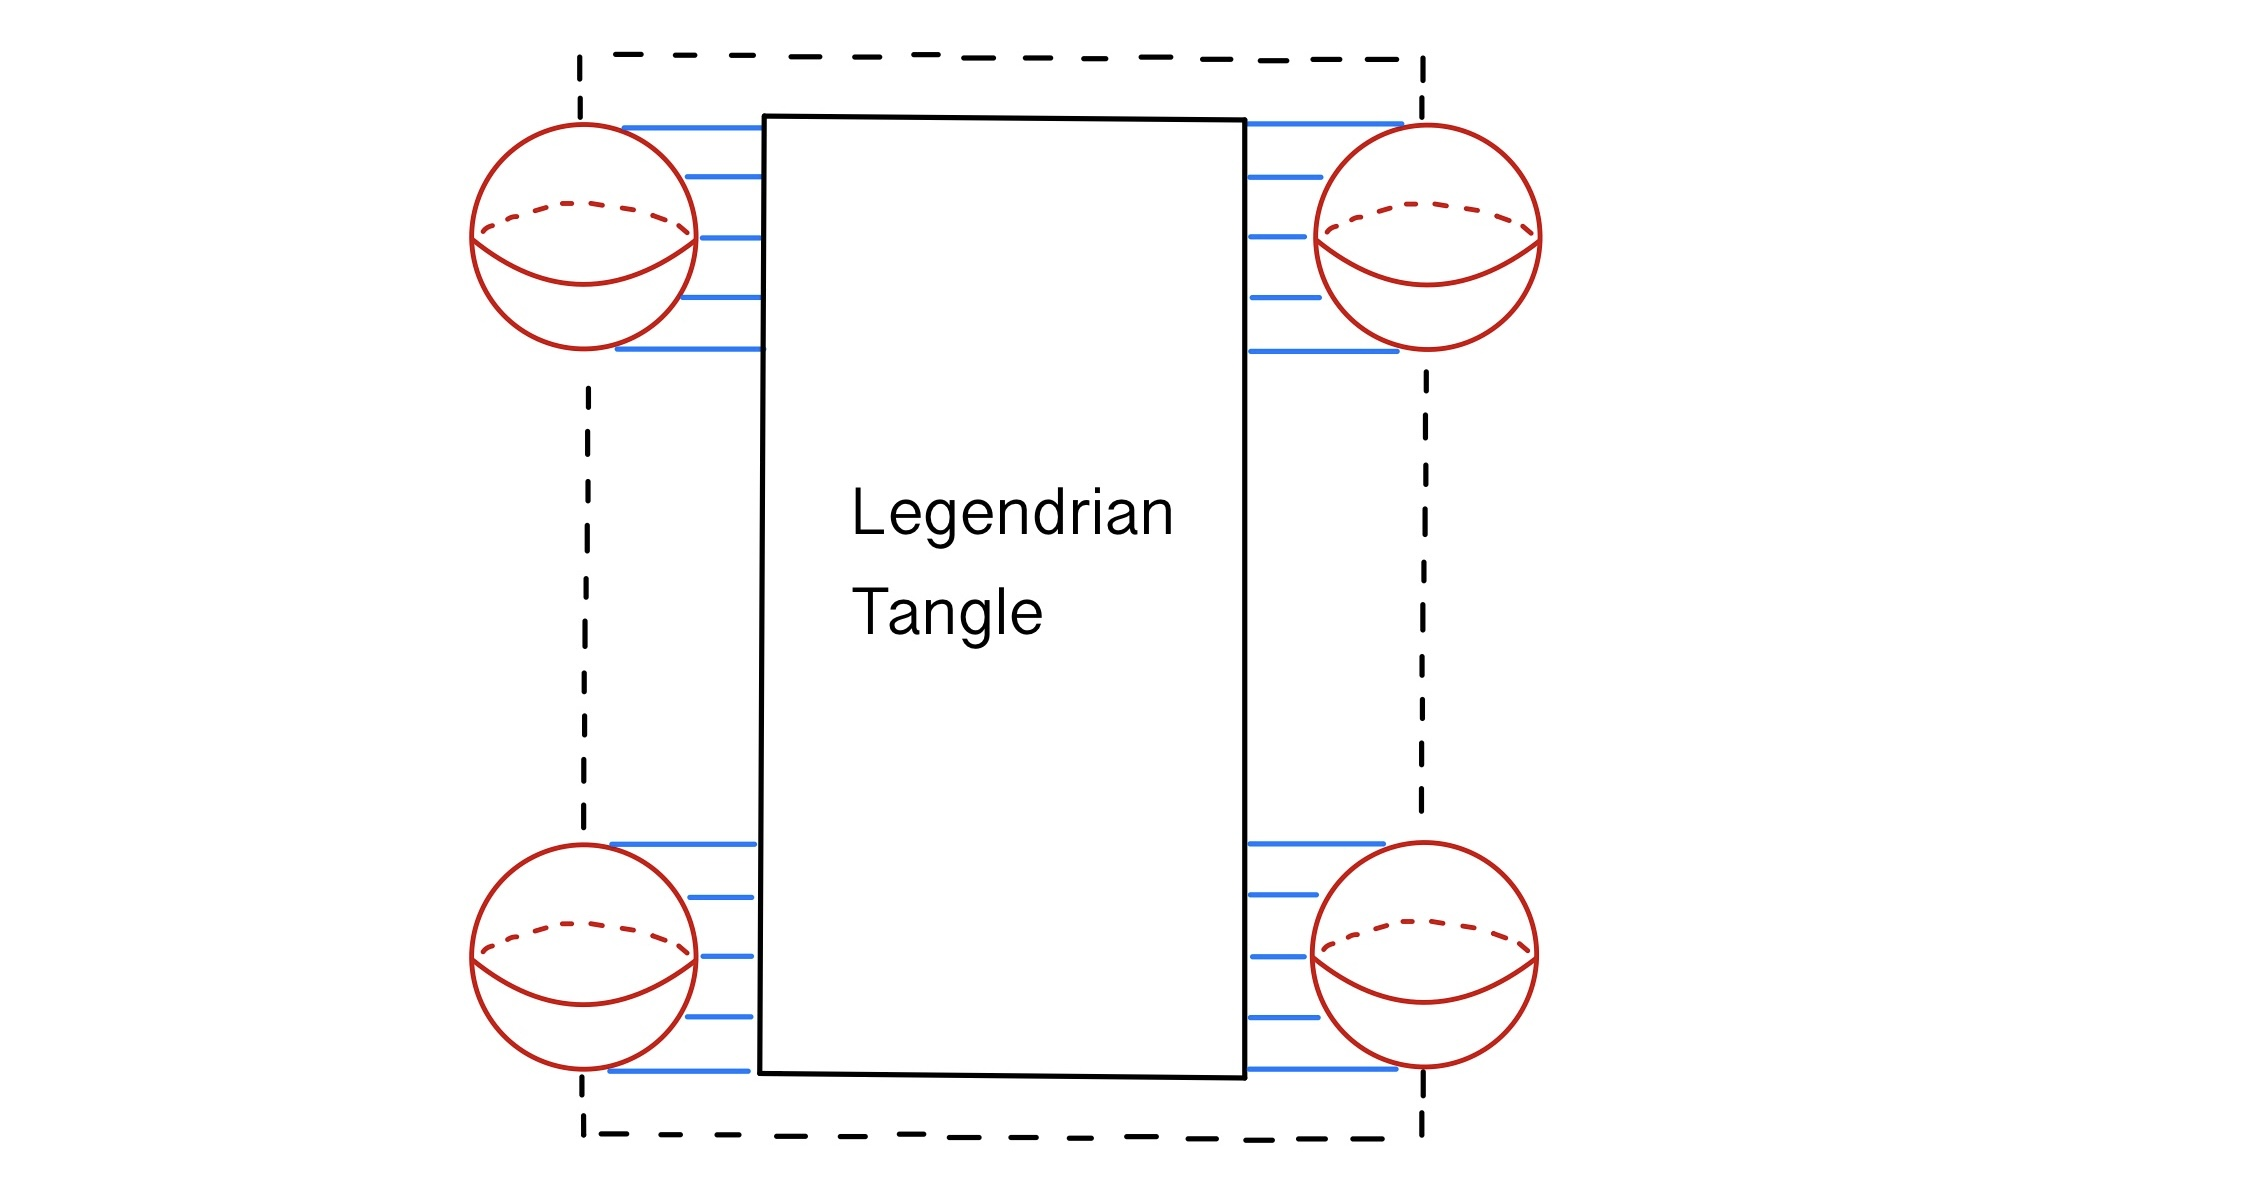
\includegraphics[scale=0.2]{figures/tango.jpeg}
    \caption{A Legendrian link in Gompf's standard form}
    \label{fig:tango}
\end{figure}
This represents a Legendrian link in $\#_1^n(\s^1 \times \s^2)$, after the $1$-handle attachment. 
We need to establish a convention to identify the framings with integers. By gluing the vertical edges of the box, the tangle becomes a link projected in the plane. Therefore, we can define the blackboard framing in the natural way. \\ Gompf shows that the well known formula for the Thurston-Bennequin invariant
$$
tb(K) = w(K)- \# \{\text{right cusps}\}
$$
is well defined for tangles in standard form, and coincides with the integer representing the contact framing \footnote{With respect to the canonical contact structure of $\#_1^n(\s^1 \times \s^2)$, determined by Eliashberg's theorem}.
Moreover, every link in $\#_1^n(\s^1 \times \s^2)$, is contact isotopic to a link in standard form. 
\begin{thm}A compact, connected $4$-manifold is Stein, if and only if, it admits a handlebody decomposition in standard form, with each $2$-handle $H_2^i$ attached to the $i^{th}$ link component $L_i$ with framing $tb(L_i)-1$.
\end{thm}


\section{Comparing Three Notions of Fillability}
In this section, we introduce three notions of symplectic fillability. They are the symplectic analogues of Stein fillability, which is the most powerful type of fillability that can be achieved.
\begin{defn}Let $(Y, \xi)$ be a contact $3$ manifold. \\
(A) $(X, \omega)$ is a weakly symplectic filling of $(Y, \xi)$ if $Y$ is the oriented \footnote{With the orientations inherited from the contact and symplectic structures} boundary of $X$ and $\omega|_{\xi}>0$. \\
(B) $(X, \omega)$ is a strongly symplectic filling of $(Y, \xi)$ if $Y$ is the oriented boundary of $X$, and there exists a contact form $\alpha$ for $\xi$, such that $\omega|_Y = d\alpha$. \\
(C) $(X, \omega)$ is said to be convex if $X$ admits a vector field $v$ that is transversely pointing outward to the boundary and Liouville, i.e. $$
\mathfrak{L}_v\omega = \omega
$$
\end{defn}
Condition (B) is clearly stronger than (A).
\begin{obs}(C) is stronger than (B). 
\end{obs}
In fact, by Cartan's formula, we have: $$
\mathfrak{L}_v\omega = d \iota_v \omega = \omega
$$ by which we can define $\alpha = \iota_v\omega$.
In general, for higher dimensional manifolds, the converse is false. However, in dimension $3/4$, one can extend a generic contact vector field transversely to the boundary, to obtain the desired Liouville vector field. For a complete discussion consult \cite{etnyre1998symplectic}, cfr \cite{Etnyre_2004}.
\begin{ex}$(\B^4, \omega_{st})$ is a convex symplectic manifold, with a Liouville vector field: $$
v = \frac{1}{2}(x\frac{\partial}{\partial x} + y\frac{\partial}{\partial y} +z\frac{\partial}{\partial z} + t\frac{\partial}{\partial t})
$$
\end{ex}
When the $3$ manifold is a homology 3-sphere, weak and strong fillability are equivalent conditions.
\begin{prop}\cite{oo:simple}\label{osha}
Let $(X, \omega)$ be a weakly symplectic filling of $(Y, \xi)$. Suppose that $\partial X = Y$ is a homology $3$ sphere. Then $\omega$ can be modified, with a small perturbation, to be a symplectic form of a strongly symplectic filling of $Y$.
\end{prop}









